The discrete Fourier transform and the FFT algorithm allow us to
efficiently implement \index{filters}{filters} with an arbitrary frequency
response. This is because the frequency domain representation of the
filter impulse response $h[n]$ can be specified as in frequency domain
$\hat{h}[k]$.

Convolution (i.e., filtering) is multiplication in frequency domain:
\begin{equation}
  \boxed{
    y[n] = h[n]\circledast x[n] \xleftrightarrow{\mathcal{F}_{D}} \hat{y}[k] = \hat{h}[k]\hat{x}[k].
    }
\end{equation}
This means that we don't even have to determine the filter impulse
response in time domain $h[n]$. One can FFT the signal $x[n]$, specify and
apply the filter $\hat{h}[k]$ directly in frequency domain through
multiplication, and finally inverse FFT the signal to obtain a
filtered signal $y[n]$.

\section{Example: Filtering out spectrally narrow frequency components}

In this example, we will create a filter that removes strong spectral
components from a signal using a band-stop filter.

Consider the following signal:
\begin{align}
  x_1[n] = &A_1\cos(\omega_1 n + \phi_1) + A_2\cos(\omega_2 n + \phi_2) \\
     & + A_3\cos(\omega_3 n + \phi_3).
\end{align}
and another signal
\begin{equation}
x_2[n] = a_1\delta[n-n_1] + a_2\delta[n - n_2] + a_3\delta[n-n_3]
\end{equation}
overlayed on top of it:
\begin{equation}
x[n] = x_1[n] + x_2[n].
\end{equation}
We'll assume that signal $x_1[n]$ is the problematic signal that we
want to filter out, so that we are able to detect the signal
$x_2[n]$. We'll assume that $|A_i| \gg |a_j|$ for all $i,j$. This
means that the signal $x_1[n]$ greatly overpowers the signal $x_2[n]$ in
amplitude. Figure \ref{fig:strong_overpowering_signal} shows $x_1[n]$,
$x_2[n]$, and $x[n]=x_1[n]+x_2[n]$ for this example. It is virtually
impossible to visually detect the weak signal $x_2[n]$ from the plot.

\begin{figure}
\begin{center}
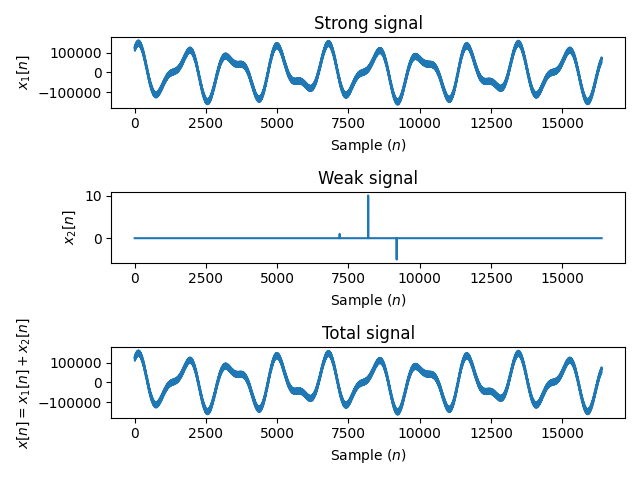
\includegraphics[width=\textwidth]{code/024_fft_filter/filter_signals.png}
\end{center}
\caption{A plot of the strong narrowband signal $x_1[n]$, the weak wideband signal $x_2[n]$, 
and the summed signal $x_1[n]+x_2[n]$. It is difficult to observe the weak signal $x_2[n]$ just by visually inspecting $x[n]$.}
\label{fig:strong_overpowering_signal}
\end{figure}

In order to detect signal $x_2[n]$, we need to filter out signal
$x_1[n]$. We can do this by creating a filter, which will remove the
strong spectral components, allowing the weak broad band signal to be
recovered. Forming such a filter in frequency domain is relatively
easy. We specify that:
\begin{equation}
\hat{h}[k] = \left\{\begin{array}{cc}
\frac{\alpha}{|\hat{x}[k]|} & \mathrm{for~strong~spectral~components}~k \\
1 & \mathrm{otherwise}
\end{array}
\right. 
\end{equation}
The strong spectral components can be identified by inspecting the
spectrum of the signal $x[n]$, that is $|\hat{x}[k]|$. When this filter is applied
in frequency domain, we obtain a frequency domain representation of the filtered signal:
\begin{equation}
\hat{y}[k] = \hat{h}[k]\hat{x}[k].
\end{equation}
The strong spectral components will be attenuated to a constant
magnitude $\alpha$, while the rest of the spectral components are
unaffected. Figure \ref{fig:example_spec_filter_strong} shows
$\hat{y}[k]$ and $\hat{x}[k]$. Note that the spectrally narrow signals
have approximately $10^{12}$ more power than the weak signals.

\begin{figure}
\begin{center}
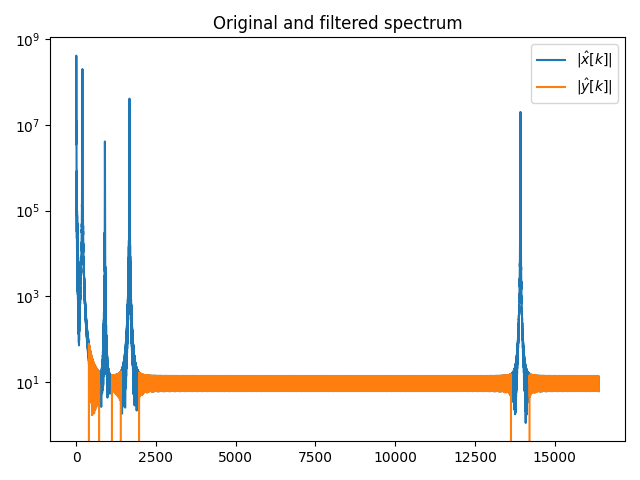
\includegraphics[width=\textwidth]{code/024_fft_filter/filter_spec.png}
\end{center}
\caption{The magnitude spectrum of signal $|\hat{x}[k]|$ and the
  magnitude spectrum of the filtered signal $|\hat{y}[k]|$. In this
  case, a logarithmic scale is used. A Hann window was applied to the
  signal when calculating the spectrum to reduce spectral leakage.}
\label{fig:example_spec_filter_strong}
\end{figure}

In order to obtain the filtered signal, we simply inverse DFT:
\begin{equation}
  y[n]=\mathcal{F}_D^{-1}\{\hat{y}[k]\}
\end{equation}
The filtered signal is shown in Figure
\ref{fig:filtered_weak_signal}. The plot shows that when strong
spectrally narrow signal components are filtered out, the weak signal
becomes visible. There are some artifacts caused by filtering, because
some spectral components of the weak signal have also been
reduced in amplitude.

In most cases, it is advantageous to use a tapered window on the signal
$x[n]$ when estimating the discrete Fourier transform, in order to reduce spectral leakage:
\begin{equation}
\hat{x}[k]= \sum_{n=0}^{N-1} w[n]x[n]e^{-\frac{2\pi}{N}nk}
\end{equation}
Here $w[n]$ would be a tapered window with better suppression of
spectral sidelobes than a rectangular window. The Hann window is one
good example.

\begin{figure}
\begin{center}
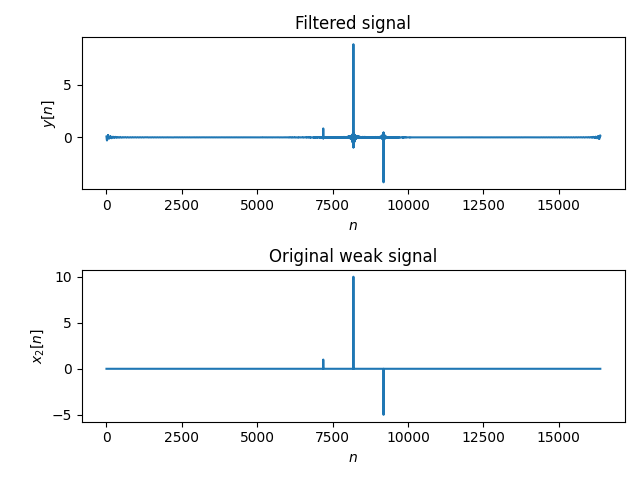
\includegraphics[width=\textwidth]{code/024_fft_filter/filter_filtered.png}
\end{center}
\caption{A comparison of the filtered estimate $y[n]$ of the weak signal $x_2[n]$ and the original signal.}\label{fig:filtered_weak_signal}
\end{figure}

The Python program used to create the plots in this example is shown
in Listing \ref{lst:fft_filter}.

\lstinputlisting[language=Python,caption={\texttt{024\_fft\_filter/fft\_filter.py}},label=lst:fft_filter]{code/024_fft_filter/fft_filter.py}


\section{Example: Whitening filter}

It is also possible to approach the previous example in a more
automatic fashion. We can also simply form a filter that whitens the
spectrum, i.e., ensures that all the spectral components are unity
magnitude after at the filter output. This is a useful filter,
especially if the signal also contains random noise. 

In this example, we'll use the same signals as we used in the previous
example. Instead of reducing the amplitudes of spectral components
within a certain range, we'll simply set the amplitudes of all
spectral components to unity:
\begin{equation}
\hat{h}[k] = \frac{1}{|\hat{x}[k]|}
\end{equation}
This type of filter is called a \index{whitening filter}{whitening filter}\sidenote{In
  statistical signal processing, $|\hat{x}[k]|$ would be replaced with
  an estimate of the mean squared spectral power
  $\sqrt{\mathrm{E}|\hat{x}[k]|^2}$. Here $\mathrm{E}$ is the
  statistical expectation operator.}

When this filter is applied in frequency domain:
\begin{equation}
\hat{y}[k] = \hat{h}[k]\hat{x}[k],
\end{equation}
the resulting signal spectrum $|\hat{y}[k]|=1$ will have a unity
magnitude at all frequencies. Figure \ref{fig:whiten_specs} shows the
spectrum of the original signal $\hat{x}[k]$ (this is the same as in
the previous example), as well as $|\hat{y}[k]|=1$.

\begin{figure}
\begin{center}
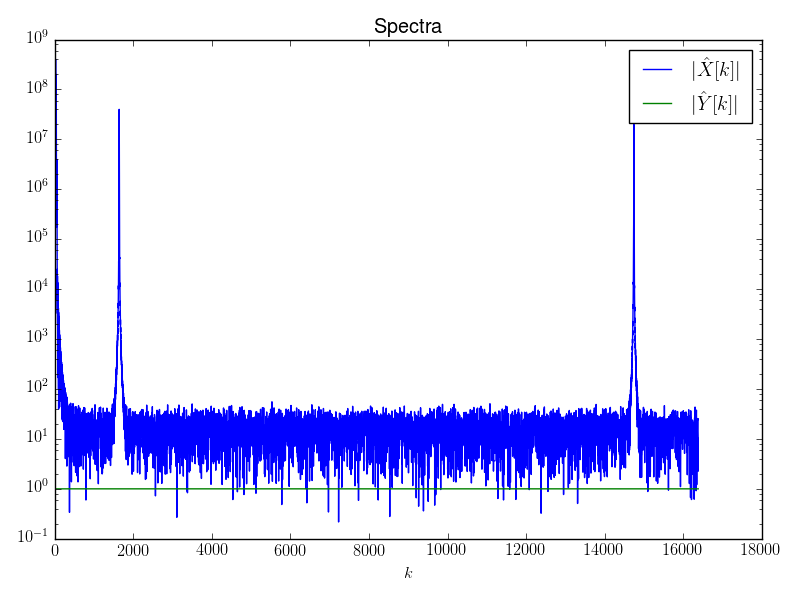
\includegraphics[width=\textwidth]{ch17/figures/whiten_spec.png}
\end{center}
\caption{Windowed magnitude spectrum of the original signal $|\hat{x}[k]|$ and the magnitude spectrum of the whitened signal $|\hat{y}[k]|$.}
\label{fig:whiten_specs}
\end{figure}

When we now inverse Fourier transform $\hat{y}[k]$, we obtain the filtered signal:
\begin{equation}
y[n] = \mathcal{F}_D^{-1}\{\hat{y}[k]\}.
\end{equation}
The filtered signal is shown in Figure \ref{fig:whitened_output}.
Note that while $|\hat{y}[k]|=1$, there is still information in the
phase $\angle \hat{y}[k]$, which allows us to detect the weak signal
$x_2[n]$.
\begin{figure}
\begin{center}
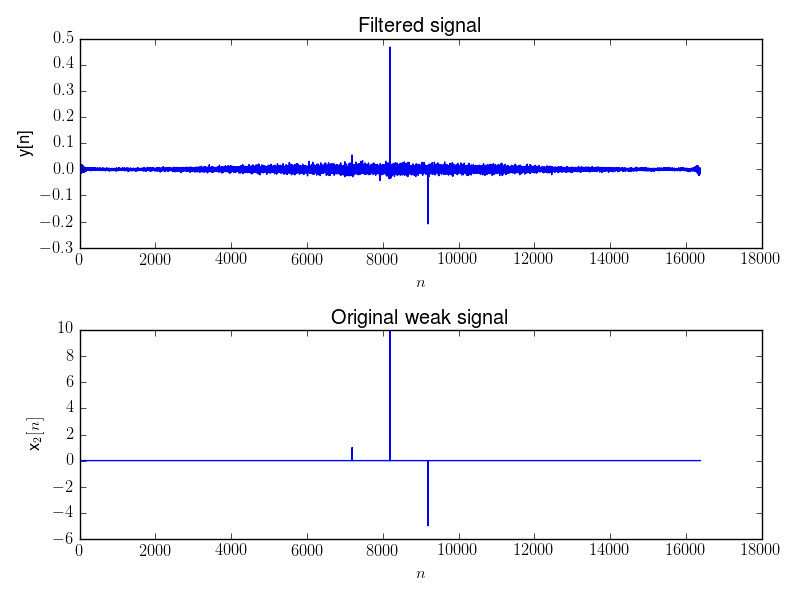
\includegraphics[width=\textwidth]{ch17/figures/whiten_filtered.png}
\end{center}
\caption{The output of the whitening filter $y[n]$. It is possible to identify the weak signal $x_2[n]$.}
\label{fig:whitened_output}
\end{figure}

The Python code used to produce this example is shown in Listing \ref{lst:whitening_filter}.

\lstinputlisting[language=Python,caption={\texttt{024\_fft\_filter/whitening\_filter.py}},label=lst:whitening_filter]{code/024_fft_filter/whitening_filter.py}

